\scanpage{92}
\mspage{22}
Par $g_n$ ce chemin devient un chemin dans $U_{03}$
\[
g_n(\widetilde\alpha_\sigma):
g_n(P')=g_n(\widetilde\sigma^0_{a_0}(P))=\tau g_n(P)=\tau(P_+)=P_-
\longrightarrow g_n(P)=P_+
\]
qui franchit l'équateur \deleted{\unsure{sur l'arc}} exactement une fois, en traversant l'arc $\widehat{(1,\infty)}$ — c'est donc $\tau_{a_1}$, noté aussi $\tau_0$ (car $a_1$ est opposé au sommet $0$) donc on trouve

\figure{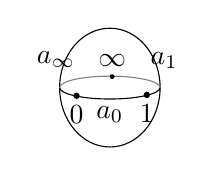
\begin{tikzpicture}[scale=.58]
\draw (0,0) ellipse (1.1 and 1.3);
\draw (-1.1,0) arc[start angle=180,end angle=360,x radius=1.1,y radius=.25];
\draw[gray] (-1.1,0) arc[start angle=180,end angle=0,x radius=1.1,y radius=.25];
\fill (-.73,-.18) circle (2pt); \node[below] at (-.73,-.18) {$0$};
\fill (.81,-.16) circle (2pt); \node[below] at (.81,-.16) {$1$};
\fill (.05,.24) circle (1.5pt); \node[above] at (.05,.24) {$\infty$};
\node[below] at (0,-.2) {$a_0$};
\node[above left] at (-.55,.22) {$a_\infty$};
\node[above right] at (.68,.2) {$a_1$};
\end{tikzpicture}}

\deleted{(99)}
\[
\tag{*} g_n(\widetilde\sigma_{a_0})=\tau_0\in
\Pi_{0,3}^{\tau}/\langle\rho_1^2,\rho_\infty^n\rangle
\]
\deleted{$\unsure{a}$}
pour se rassurer on vérifiera que conformément à (86), $\widetilde\sigma_{a_0}(\rho)=\rho^{-1}$, $\widetilde\sigma_{a_0}(\sigma_{a_0})=\sigma_{a_0}$, on a bien
\[
\tau_0(\rho_\infty^{-1})=\rho_\infty^{\deleted{\unsure{-1}}},\quad
\tau_0(\rho_1)=\rho_1^{-1}
\]
ce qui est contenu en effet dans les (deux premières) formules (80) pour $n=3$, en prenant ici pour $a_0$ le côté $(1,\infty)$ du triangle $(0,1,\infty)$ \deleted{\unsure{dans}} dans $X_0$ \ldots. On tire de \deleted{(99)} (*)
\[
g_n(\tau_{a_0})=g_n(\widetilde\sigma_{a_0}.\sigma_{a_0})
=g_n(\widetilde\sigma_{a_0})g_n(\sigma_{a_0})
=\tau_0\rho_1=\tau_\infty
\]
puisque $\rho_1=\tau_0\tau_\infty$, \deleted{donc} en résumé
\[
\tag{100}
g_n(\widetilde\sigma_{a_0})=\tau_0,\quad g_n(\tau_{a_0})=\tau_\infty.
\]

\figure{\begin{tikzpicture}\draw (0,.6)--(.55,0);\end{tikzpicture}}

7: Dans toutes ces considérations, \inserted{du § 6} on a un peu perdu de vue les cartes, dont il n'a plus été question. Pourtant, le groupe $\Pi_P^\tau$ s'interprète comme le groupe ``cartographique pondéré $\unsure{n}$-polygonal'', qui est tel que

\margin{91}
